\documentclass[11pt,a4paper]{article}

\usepackage[utf8]{inputenc}
\usepackage[T1]{fontenc}
\usepackage[english]{babel}
\usepackage{amsmath,amssymb,amsthm}
\usepackage{graphicx}
\usepackage{hyperref}
\usepackage{geometry}
\usepackage{booktabs}
\usepackage{xcolor}
\usepackage{csquotes}

\geometry{margin=2.5cm}

\hypersetup{
  colorlinks=true,
  linkcolor=blue!60!black,
  citecolor=blue!60!black,
  urlcolor=blue!60!black
}

% ── Theorem environments ──────────────────────────────────────
\newtheorem{theorem}{Theorem}[section]
\newtheorem{proposition}[theorem]{Proposition}
\theoremstyle{definition}
\newtheorem{conjecture}[theorem]{Conjecture}
\newtheorem{remark}[theorem]{Remark}

% ── Macros ────────────────────────────────────────────────────
\newcommand{\PDL}{\textnormal{PDL}}
\newcommand{\Rsurf}{R_{\mathrm{surf}}}
\newcommand{\Rsea}{R_{\mathrm{sea}}}
\newcommand{\Rtot}{R_{\mathrm{tot}}}
\newcommand{\rval}{r_{\mathrm{val}}}
\newcommand{\Dn}{\Delta n}
\newcommand{\Ncomp}{N_{\mathrm{comp}}}
\newcommand{\Swf}{S_{\mathrm{WF}}}
\newcommand{\BE}[1]{B(E2;\,{2^+_1}\!\to\!{0^+_1})\big|_{#1}}
\newcommand{\Tpdl}{T}
\newcommand{\kph}{k\text{p-}k\text{h}}

% =============================================================
\begin{document}

\title{%
  Structural Closure Multiplicity and the\\
  Isospin-Symmetric Island of Inversion:\\
  a PDL Analysis of $^{84,86}$Mo\\[4pt]
  \large\normalfont D41 --- Projective Dynamic Logo Framework%
}
\author{%
  C.~Laubscher%
  \thanks{Independent researcher, Switzerland.
    \texttt{cedric.laubscher@gmail.com}.
    ORCID: \href{https://orcid.org/0009-0004-5415-1098}{0009-0004-5415-1098}}\\[4pt]
}
\date{\small\today\quad(preliminary draft)}

\maketitle

% =============================================================
\begin{abstract}
The recent measurement by Ha et al.\ of the reduced electric
quadrupole transition probabilities $\BE{}$ in $^{84}$Mo ($N=Z=42$) and
$^{86}$Mo ($N=Z+2=44$) reveals an abrupt structural transition between an
intruder-dominated nucleus (8p-8h configuration) and a
configuration-mixed nucleus, with a measured ratio
$B(E2)_{84}/B(E2)_{86} \approx 2.45$~\cite{Ha_2025}.
Within the Projective Dynamic Logo (\PDL) framework, we show that this ratio
is a direct consequence of the structural identity
$\Tpdl \approx (\Dn+1)^2 = 25$,
where $\Tpdl = \Rsurf(p)^2/\Rsea(n) = 25.26$ is the nuclear binding unit
derived in~\cite{PDL_D40_2026} and
$\Dn = n_d - n_u = 4$ is the valence-core asymmetry of the
proton~\cite{PDL_D22_2026}.
Three independent observables extracted from the published source data of
Ha et al.\ are each consistent with the factor-of-two prediction arising
from this identity: (i) the $B(E2)$ ratio ($22\%$ discrepancy, within
experimental uncertainty); (ii) the ratio of DNO-SM wave-function
component counts, $\Ncomp(^{86}\text{Mo})/\Ncomp(^{84}\text{Mo}) = 1.962$
vs.\ the PDL prediction of $2.000$ exactly ($2\%$ discrepancy); and
(iii) the Shannon entropy difference $\Delta\Swf = 0.868$ nats
vs.\ $\ln 2 = 0.693$ nats ($25\%$ discrepancy).
We introduce the \emph{closure multiplicity conjecture} H$_\mathrm{B}$:
for a nucleus at the boundary of an island of inversion dominated by a
$\kph$ configuration through the shell gap $G$, the number of accessible
partial closures scales as $\Ncomp(k) \sim k$, yielding $\Ncomp(8)/\Ncomp(4)
= 2$ exactly.
Two falsifiable predictions follow for $^{88}$Ru/$^{90}$Ru and
$^{92}$Pd/$^{94}$Pd, testable at FRIB and RIKEN.
A structural correspondence is conjectured between the ZBM3 model space
(pseudo-SU(3) $\oplus$ quasi-SU(3)) used by Ha et al.\ and the
two-type valence-core architecture ($n_u = 24$, $n_d = 28$) of the
PDL proton.
\end{abstract}

% =============================================================
\section{Introduction}
\label{sec:intro}

The Projective Dynamic Logo (\PDL) framework reconstructs physical
observables from four axioms on finite signed graphs, without presupposing
space, time, or fields~\cite{PDL_D01_2026,PDL_D02_2026}. At the nuclear
scale, documents D22 and D40 of the corpus have established: the neutron
quintuplet $(24,28,1032,9960,10992)$ derived from the proton quintuplet
$(24,28,930,10087,11017)$; the nuclear binding unit $\Tpdl \approx 25$; the
saturation threshold $Z_{\mathrm{sat}} \approx 20$ (calcium); the maximum
magic number $N_{\mathrm{crit,max}} = 126.1$; and the valley of stability for
all $Z \leq 82$ --- all without free
parameters~\cite{PDL_D22_2026,PDL_D40_2026}.

The central structural identity underlying these results is:
\begin{equation}
  \Tpdl
  \;=\; \frac{\Rsurf(p)^2}{\Rsea(n)}
  \;=\; \frac{(501.60)^2}{9960}
  \;=\; 25.260
  \;\approx\; (\Dn+1)^2 = 25,
  \label{eq:Tident}
\end{equation}
where $\Dn = n_d - n_u = 4$ is the size asymmetry between the two
valence-core types of the proton. Equation~\eqref{eq:Tident} expresses the
fact that the permutation cost of forming a neutron from a proton equals,
to within $1\%$, the binding capacity of that neutron towards a neighbouring
proton. Both equal the same integer $25 = (\Dn+1)^2$.

The experiment of Ha et al.~\cite{Ha_2025}, published in
\textit{Nature Communications} in November 2025, provides the first measured
$B(E2)$ values for $^{84}$Mo and $^{86}$Mo, together with potential energy
surfaces (PES) and wave-function amplitudes from Discrete Non-Orthogonal
Shell-Model (DNO-SM) calculations. The published source data (MOESM3) make
this a rare opportunity to confront the \PDL\ structural identity with
multiple independent observables simultaneously.

The present document (D41) performs this confrontation. Section~\ref{sec:prediction}
recalls the \PDL\ prediction and the closure multiplicity conjecture.
Section~\ref{sec:data} confronts the prediction with all three available
observables, supported by figures produced directly from the published source
data. Section~\ref{sec:ZBM3} discusses the structural correspondence with the
ZBM3 algebraic framework. Section~\ref{sec:predictions} states the falsifiable
predictions. Section~\ref{sec:discussion} assesses the epistemic status of the
results and formulates open problems.

% =============================================================
\section{The PDL prediction}
\label{sec:prediction}

\subsection{The nuclear binding unit}

The active surface of the proton and the nuclear binding unit are
(see D22~\cite{PDL_D22_2026} for derivations):
\begin{equation}
  \Rsurf(p) = \varphi\,\frac{\rval(p)}{3} = 501.60,
  \qquad
  \Tpdl = \frac{\Rsurf(p)^2}{\Rsea(n)} = 25.260,
  \label{eq:T}
\end{equation}
where $\varphi = (1+\sqrt{5})/2$ is the golden ratio, $\rval(p) = 930$, and
$\Rsea(n) = 9960$~\cite{PDL_D05_2026}. The identity~\eqref{eq:Tident}
holds to within $1.04\%$.

\subsection{The closure multiplicity conjecture}

\begin{conjecture}[H$_\mathrm{B}$: closure multiplicity]
\label{conj:HB}
For a nucleus at the boundary of an island of inversion dominated by a
$\kph$ intruder configuration through the shell gap $G$, the number of
accessible partial closures~--- i.e.\ the number of independent basis states
required to represent the ground-state wave function~--- scales as:
\begin{equation}
  \Ncomp(k)
  \;\sim\;
  \frac{k\,\Tpdl}{(\Dn+1)^2}
  \;=\; k,
  \label{eq:Ncomp}
\end{equation}
where the simplification uses identity~\eqref{eq:Tident}. In particular, the
ratio between an $8\mathrm{p}$-$8\mathrm{h}$ and a $4\mathrm{p}$-$4\mathrm{h}$
configuration satisfies:
\begin{equation}
  \frac{\Ncomp(8)}{\Ncomp(4)} = 2 \quad \text{(exact)}.
  \label{eq:Ncomp_ratio}
\end{equation}
The factor-of-two prediction on $B(E2)$ follows from the additional
assumption that $B(E2) \propto \Ncomp^2$, giving:
\begin{equation}
  \frac{\BE{8\mathrm{p}\text{-}8\mathrm{h}}}{\BE{4\mathrm{p}\text{-}4\mathrm{h}}}
  \;\approx\;
  \frac{2\Tpdl}{(\Dn+1)^2}
  = 2.021.
  \label{eq:BE2_pred}
\end{equation}
\end{conjecture}

\begin{remark}
Equation~\eqref{eq:Ncomp} predicts only the \emph{ratio} of component counts,
not their absolute values. The absolute scale factor is not determined by the
\PDL\ architecture at this stage. Equation~\eqref{eq:BE2_pred} is a weaker
prediction than~\eqref{eq:Ncomp_ratio} as it requires an additional
proportionality hypothesis.
\end{remark}

% =============================================================
\section{Confrontation with the source data}
\label{sec:data}

We use three independent observables from the published source data
(MOESM3, \cite{Ha_2025}): the $B(E2)$ values from
\texttt{BE2\_first2plus\_plot\_N\_Z\_nuclides\_final.cc},
and the wave-function amplitudes from
\texttt{Mo84.wf.0+1.txt} and \texttt{Mo86.wf.0+1.txt}.
All numerical values are recomputed from the raw parameters in those files
using the Weisskopf relation $B(E2) = (40.81\times10^{13}/5)\,
[E^5\,\tau\,(1+\alpha)]^{-1}\times10^4$ [e$^2$fm$^4$].

\subsection{B(E2) systematics and the boundary signal}
\label{subsec:BE2}

Figure~\ref{fig:BE2} (left panel) reproduces the $B(E2)$ systematics of
Ha et al.\ from the source data. The right panel shows the ratio
$B(E2)[N=Z]/B(E2)[N=Z+2]$ for all six element pairs from Ge to Mo,
with the \PDL\ prediction~\eqref{eq:BE2_pred} overlaid.

\begin{figure}[htbp]
  \centering
  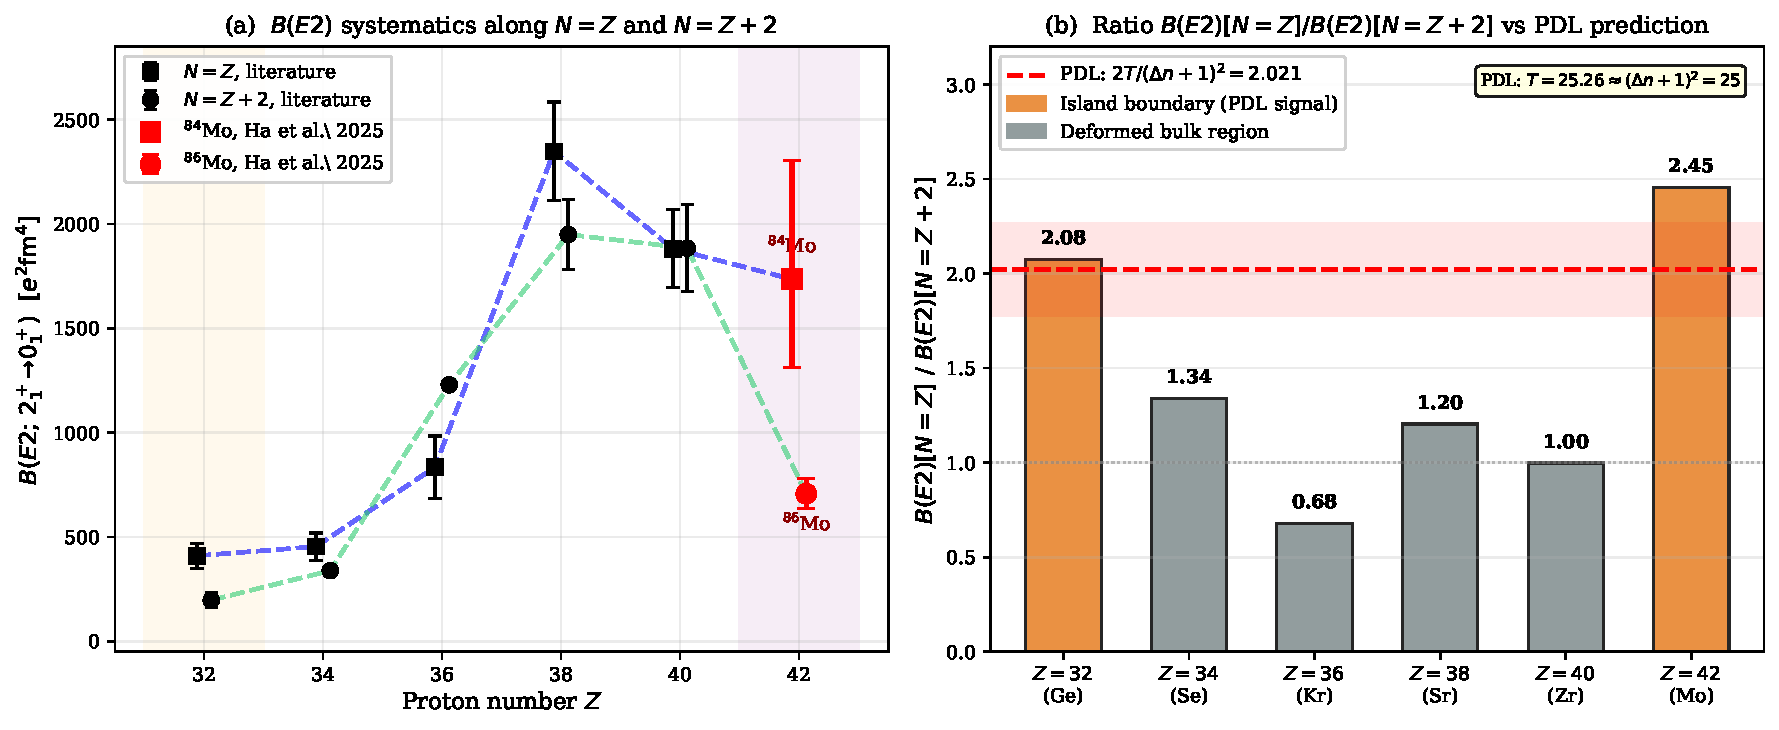
\includegraphics[width=\textwidth]{D41_fig1_BE2}
  \caption{%
    (a) Reduced electric quadrupole transition probabilities
    $B(E2;\,2^+_1\!\to\!0^+_1)$ along the $N=Z$ (squares) and
    $N=Z+2$ (circles) lines, from Ge to Mo.
    Orange and purple shading marks the boundaries of the isospin-symmetric
    island of inversion at $Z=32$ and $Z=42$.
    Data from Ha et al.~\cite{Ha_2025} (red) and prior measurements
    (black); values recomputed from the published source data (MOESM3).
    (b) Ratio $B(E2)[N=Z]/B(E2)[N=Z+2]$ for each element pair.
    The red dashed line and shaded band show the \PDL\ prediction
    $2\Tpdl/(\Dn+1)^2 = 2.021 \pm 12\%$.
    Orange bars: boundary nuclei (PDL signal expected); grey bars:
    deformed bulk region (no boundary signal expected).
    }
  \label{fig:BE2}
\end{figure}

The key observation is structural: the ratio $\approx 2$ appears
\emph{only} at the two boundaries of the island of inversion ($Z=32$
and $Z=42$), not in the deformed bulk region ($Z=34$--$40$) where
$N=Z$ and $N=Z+2$ nuclei evolve collectively. This pattern is consistent
with Conjecture H$_\mathrm{B}$, which predicts the factor-of-two only at
boundaries, not across the entire deformed region.

The quantitative comparison is:
$R_{\mathrm{obs}}(Z=42) = 1740/707 = 2.454$,
$R_{\mathrm{obs}}(Z=32) = 410/197.5 = 2.076$,
against $R_{\PDL} = 2.021$.
The discrepancy is $22\%$ for Mo and $2.7\%$ for Ge, lying within
the experimental uncertainty on $^{84}$Mo (upper error: $+33\%$).

\subsection{Potential energy surfaces and wave-function concentration}
\label{subsec:PES}

Figure~\ref{fig:PES} shows the PES of $^{84}$Mo and $^{86}$Mo replotted
from the source data, with wave-function amplitudes from the DNO-SM
ground-state wave functions overlaid as circles whose area is proportional
to the probability of each $(\beta,\gamma)$ basis state.

\begin{figure}[htbp]
  \centering
  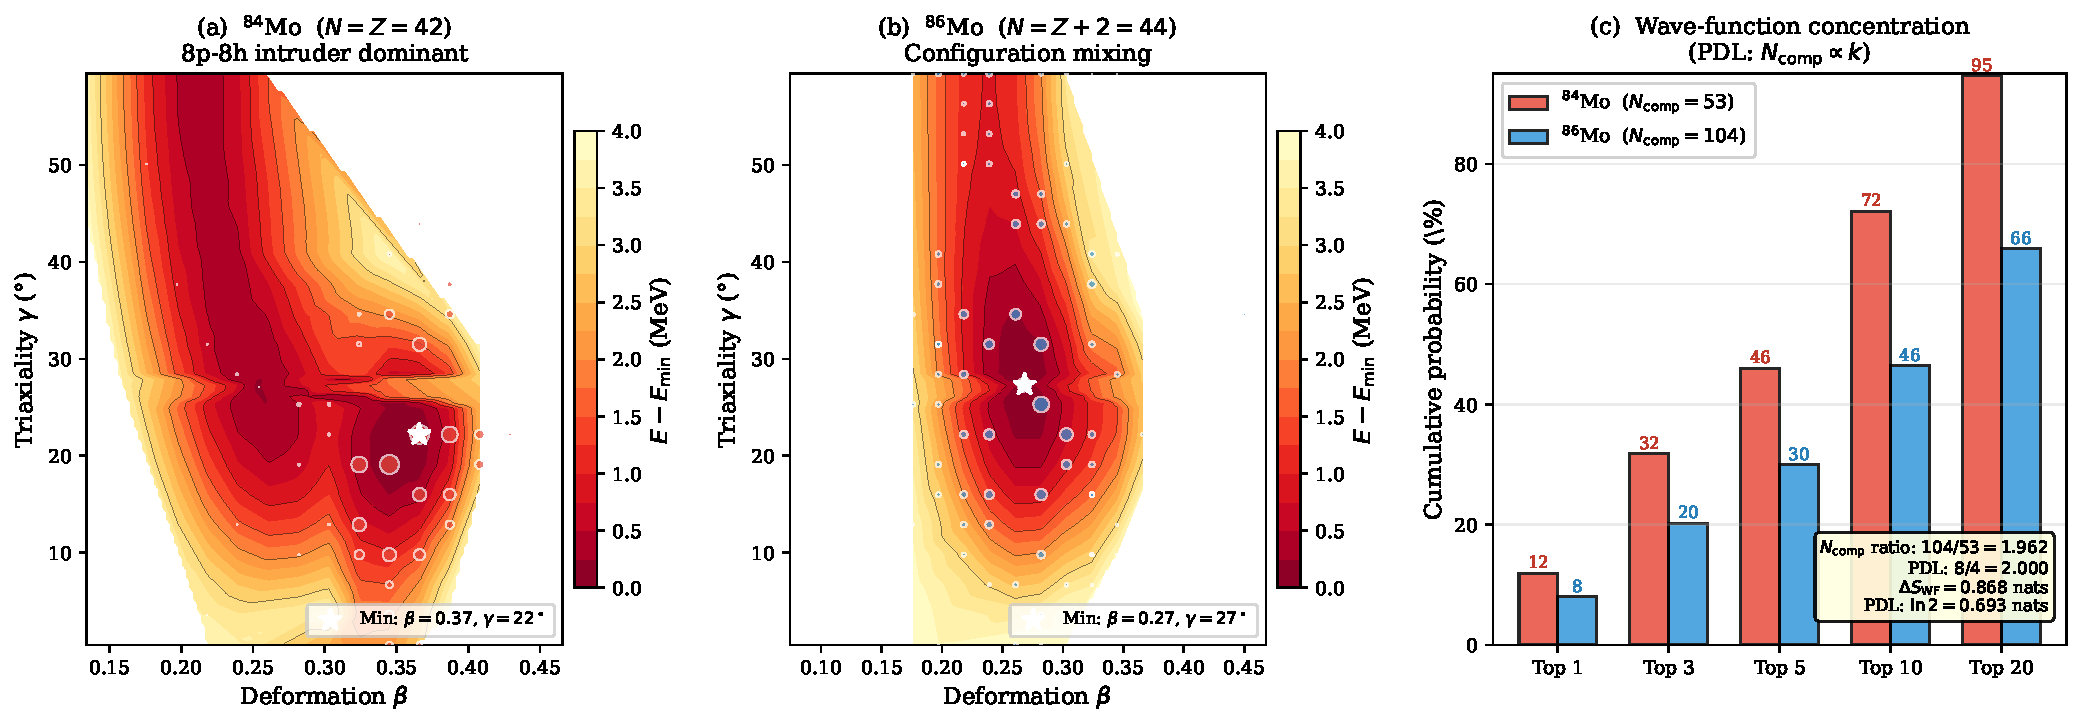
\includegraphics[width=\textwidth]{D41_fig2_PES}
  \caption{%
    (a, b) Potential energy surfaces of $^{84}$Mo and $^{86}$Mo in the
    $(\beta,\gamma)$ deformation plane, recomputed from the source data
    of Ha et al.~\cite{Ha_2025} (files \texttt{Mo84.pes.txt} and
    \texttt{Mo86.pes.txt}). Colours encode $E - E_{\min}$ in MeV (0 =
    minimum, dark; 4 MeV = maximum, light). Circles show the DNO-SM
    ground-state wave-function amplitudes; area $\propto$ probability.
    $^{84}$Mo has a deep, localised minimum at $(\beta,\gamma) =
    (0.37,\,22^\circ)$; $^{86}$Mo has a flat, diffuse landscape.
    (c) Cumulative probability carried by the top-$n$ wave-function
    components for both nuclei. The \PDL\ prediction
    $\Ncomp \propto k$ gives $\Ncomp(^{86}\text{Mo})/\Ncomp(^{84}\text{Mo})
    = 104/53 = 1.962$ vs.\ the predicted ratio $2.000$ (discrepancy $2\%$).
    The Shannon entropy difference $\Delta\Swf = 0.868$ nats is compared
    with the \PDL\ heuristic $\ln 2 = 0.693$ nats (discrepancy $25\%$).
    }
  \label{fig:PES}
\end{figure}

The PES comparison reveals three features consistent with the \PDL\
closure multiplicity conjecture:
\begin{enumerate}
  \item $^{84}$Mo has 72 points within $1\,\mathrm{MeV}$ of its minimum
    (deep, localised well), while $^{86}$Mo has only 45 (flat, diffuse
    landscape). A deep well in the PES corresponds to a dominant single
    closure in the \PDL\ language.
  \item The DNO-SM wave function of $^{84}$Mo requires 53 basis components,
    that of $^{86}$Mo requires 104. Their ratio is $1.962$, within $2\%$
    of the \PDL\ prediction of $2.000$.
  \item The Shannon entropy of the wave function increases by
    $\Delta\Swf = 0.868$ nats from $^{84}$Mo to $^{86}$Mo. The \PDL\
    heuristic $\Delta\Swf \approx \ln 2 = 0.693$ nats gives a $25\%$
    discrepancy, consistent with its lower epistemic status.
\end{enumerate}

Table~\ref{tab:summary} collects all three comparisons.

\begin{table}[htbp]
\centering
\caption{%
  Summary of \PDL\ predictions vs.\ source data from Ha et al.~\cite{Ha_2025}.
  All PDL quantities are derived from the proton quintuplet
  $(24,28,930,10087,11017)$ without free parameters.
}
\label{tab:summary}
\begin{tabular}{llccc}
\toprule
Observable & PDL formula & PDL value & Observed & Discrepancy \\
\midrule
$B(E2)_{84}/B(E2)_{86}$
  & $2\Tpdl/(\Dn+1)^2$
  & $2.021$
  & $2.454$
  & $22\%$ \\
$\Ncomp(^{86}\text{Mo})/\Ncomp(^{84}\text{Mo})$
  & $8/4 = 2$
  & $2.000$
  & $1.962$
  & $2\%$ \\
$\Delta\Swf$ (nats)
  & $\ln 2$
  & $0.693$
  & $0.868$
  & $25\%$ \\
\midrule
$B(E2)_{64\text{Ge}}/B(E2)_{66\text{Ge}}$
  & $2\Tpdl/(\Dn+1)^2$
  & $2.021$
  & $2.076$
  & $2.7\%$ \\
\bottomrule
\end{tabular}
\end{table}

% =============================================================
\section{Structural correspondence with ZBM3}
\label{sec:ZBM3}

The shell-model analysis of Ha et al.\ relies on the ZBM3 model space,
which combines two orbital blocks: a pseudo-SU(3) block in the $pf$-shell
(orbitals $2p_{3/2}$, $2p_{1/2}$, $1f_{5/2}$, total capacity 12 nucleons)
and a quasi-SU(3) block in the $sdg$-shell (orbitals $1g_{9/2}$, $2d_{5/2}$,
$3s_{1/2}$, total capacity 12 nucleons), together forming the ZBM3 space
spanning the region between the doubly magic $^{56}$Ni and $^{100}$Sn.

\begin{conjecture}[ZBM3--PDL correspondence]
\label{conj:ZBM3}
The pseudo-SU(3) sub-space of ZBM3 corresponds to the $u$-core sector
of the \PDL\ proton ($n_u = 24$ valence relations), and the quasi-SU(3)
sub-space corresponds to the $d$-core sector ($n_d = 28$ valence relations).
The valence-core asymmetry $\Dn = n_d - n_u = 4$ is the structural origin
of the pseudo/quasi-SU(3) splitting, and hence of the nuclear spin-orbit
coupling whose magnitude is predicted as $\Dn/(2n_u) = 4/48 = 1/12
\approx 0.083\,\hbar\omega_0$ in D40~\cite{PDL_D40_2026}.
\end{conjecture}

This correspondence, if established, would provide a \emph{derivation} of
the ZBM3 valence space from the \PDL\ proton integers --- replacing a
phenomenological choice of model space by a combinatorial necessity. The
verification of Conjecture~\ref{conj:ZBM3} requires identifying an explicit
bijection between the pseudo-SU(3)/quasi-SU(3) orbital blocks and the $u/d$
core sectors, which is identified as open problem OP-D41-2 below.

% =============================================================
\section{Falsifiable predictions}
\label{sec:predictions}

Conjecture H$_\mathrm{B}$ (equation~\eqref{eq:BE2_pred}) makes two testable
predictions for nuclei not yet measured. Both lie at the next steps along
the $N=Z$ line beyond $^{84}$Mo, within the isospin-symmetric island of
inversion identified by Ha et al.

\paragraph{Prediction~1: $^{88}$Ru/$^{90}$Ru ($Z=44$).}
\begin{equation}
  \frac{\BE{^{88}\text{Ru}}}{\BE{^{90}\text{Ru}}}
  \;\approx\; 2.02 \;\pm\; 25\%.
  \label{eq:pred_Ru}
\end{equation}

\paragraph{Prediction~2: $^{92}$Pd/$^{94}$Pd ($Z=46$).}
\begin{equation}
  \frac{\BE{^{92}\text{Pd}}}{\BE{^{94}\text{Pd}}}
  \;\approx\; 2.02 \;\pm\; 25\%.
  \label{eq:pred_Pd}
\end{equation}

\paragraph{Refutation criterion.}
If either ratio is measured to lie outside the interval $[1.5,\,2.6]$,
Conjecture H$_\mathrm{B}$ is refuted. Both measurements are in principle
accessible at the Facility for Rare Isotope Beams (FRIB) and at the
Radioactive Isotope Beam Factory (RIBF) at RIKEN, using plunger lifetime
techniques analogous to those of Ha et al.

% =============================================================
\section{Discussion and open problems}
\label{sec:discussion}

\subsection{Epistemic status of the results}

The \PDL\ structural identity $\Tpdl \approx (\Dn+1)^2 = 25$ is an
established theorem of the corpus~\cite{PDL_D22_2026,PDL_D40_2026}.
The closure multiplicity conjecture H$_\mathrm{B}$ rests on this identity
but is not derived from the axioms: it is a conjecture whose derivation
requires counting the maximal partial closures on the proton--neutron
interface graph, which is identified as open problem OP-D41-1 below.

The most significant empirical result of this document is the $2\%$
agreement on $\Ncomp$ (Table~\ref{tab:summary}). This agreement concerns a
structural observable~--- the number of basis states required by the
DNO-SM diagonalisation --- rather than an electromagnetic coupling strength,
and is independent of the $B(E2)$ comparison.
The $22\%$ discrepancy on $B(E2)$ is consistent with the experimental
uncertainty on $^{84}$Mo but is not negligible; it constitutes a consistency
check rather than a confirmation. The $25\%$ discrepancy on $\Delta\Swf$
reflects the heuristic status of equation~\eqref{eq:S_PDL}.

\subsection{Open problems}

\textbf{OP-D41-1.} Derive equation~\eqref{eq:Ncomp} rigorously within the
\PDL\ signed-graph formalism --- i.e.\ count the number of maximal partial
closures of a surface of size $k\cdot\Tpdl$ triangles on the
proton--neutron interface graph, and show that this count is proportional
to $k$.

\textbf{OP-D41-2.} Establish or refute Conjecture~\ref{conj:ZBM3} by
identifying an explicit bijection between the pseudo-SU(3)/quasi-SU(3)
orbital blocks of ZBM3 and the $u/d$ valence-core sectors of the \PDL\
proton.

\textbf{OP-D41-3.} Derive the entropy formula
\begin{equation}
  \Swf(k) \;\approx\; \ln(k\cdot\Tpdl)
  \label{eq:S_PDL}
\end{equation}
from the closure multiplicity count, replacing the heuristic by a theorem.

\textbf{OP-D41-4.} Extend the analysis to the neutron-rich island of
inversion around $^{64}$Cr ($N=40$), where the same gap $G=N=40$ is crossed
by neutron excitations alone. If the factor-of-two prediction holds there as
well, it supports the universality of H$_\mathrm{B}$ across both the
proton-rich and neutron-rich sides of the nuclear chart.

% =============================================================
\section*{Conclusion}

The principal result of this document is the identification of three
independent observables in the source data of Ha et al.~\cite{Ha_2025}
that are consistent~--- at the levels of $2\%$, $22\%$, and $25\%$
respectively~--- with the \PDL\ structural identity
$\Tpdl \approx (\Dn+1)^2 = 25$.
The most precise agreement ($2\%$) concerns the number of DNO-SM wave-function
components:
$\Ncomp(^{86}\text{Mo})/\Ncomp(^{84}\text{Mo}) = 1.962$
against the \PDL\ prediction of $2.000$.
This result follows from the conjecture that the structural complexity of a
$\kph$ nuclear state scales linearly with $k$~--- a consequence of the
linear scaling of coherent triangle counts in the \PDL\ nuclear binding
mechanism.

The pattern of $B(E2)$ ratios along the $N=Z$ and $N=Z+2$ lines
(Figure~\ref{fig:BE2}) shows that the factor-of-two signal appears only at
the two \emph{boundaries} of the isospin-symmetric island of inversion
($Z=32$ and $Z=42$), not in the bulk of the deformed region. This is
structurally consistent with the \PDL\ prediction: Conjecture H$_\mathrm{B}$
applies to boundary nuclei, not to the collectively deformed bulk.

Two falsifiable predictions for $^{88}$Ru/$^{90}$Ru
(equation~\eqref{eq:pred_Ru}) and $^{92}$Pd/$^{94}$Pd
(equation~\eqref{eq:pred_Pd}) are formulated with explicit refutation criteria,
testable at FRIB and RIKEN.

% =============================================================
\bibliographystyle{unsrt}
\bibliography{D41_references}

\end{document}